\chapter{Implémentation}


\chapteropeningtext{Après avoir présenté la conception générale de SomaScan, ce chapitre décrit la phase d'implémentation de la solution. Il montre comment les choix de conception ont été traduits en éléments techniques concrets au niveau du backend Laravel, de l'application mobile Flutter et de l'application web React.\par\medskip Contrairement au chapitre précédent, qui présente les choix d'architecture, ce chapitre se concentre sur la réalisation pratique : organisation des projets, modules implémentés, logique métier principale, intégration des API, gestion de l'authentification et validation des principales interfaces. Les captures et illustrations finales seront ajoutées sous forme de figures lorsque les écrans et les tests seront documentés.}{Implémentation -- Backend Laravel -- Mobile Flutter -- Web React -- API -- Tests}

\section{Environnement de développement et outils}

Le développement de SomaScan a reposé sur trois applications complémentaires. Le backend Laravel centralise la logique métier et expose les API REST. L'application mobile Flutter permet aux opérateurs terrain de scanner les camions. L'application web React permet à l'agent logistique d'administrer les données, de suivre les trajets et de préparer les rapports.

L'environnement utilisé pour le développement et la validation locale ne correspond pas encore à l'environnement de production. Il sert principalement à implémenter les fonctionnalités, tester les échanges entre les trois applications et vérifier les scénarios métier avant le déploiement. Cette configuration locale est la suivante :

\begin{itemize}
    \item le backend Laravel est exécuté sur le serveur local de développement Laravel ;
    \item la base de données est exécutée localement à travers XAMPP ;
    \item l'application mobile Flutter est exécutée sur un téléphone Android réel avec le mode débogage activé ;
    \item l'application web React est exécutée avec le serveur de développement Vite.
\end{itemize}

Les aspects liés au serveur de production, à la configuration réseau finale et au processus de déploiement seront traités séparément dans le chapitre~5.

Les principaux outils et technologies utilisés sont présentés dans le tableau~\ref{tab:outils-implementation}.

\begin{table}[H]
\centering
\begin{tabularx}{\textwidth}{|p{4cm}|X|}
\hline
\textbf{Partie} & \textbf{Technologies et outils utilisés} \\
\hline
Backend & Laravel, PHP, serveur local Laravel, API REST, Laravel Sanctum, Eloquent ORM, base de données locale avec XAMPP. \\
\hline
Application mobile & Flutter, Dart, Riverpod, GoRouter, Dio, Flutter Secure Storage, Mobile Scanner, exécution sur téléphone Android réel en mode débogage. \\
\hline
Application web & React, TypeScript, serveur de développement Vite, React Router DOM, Zustand, Axios, Tailwind CSS, Recharts, qrcode, jsPDF. \\
\hline
Validation & Tests manuels, appels API, vérification des scénarios de scan, contrôle des erreurs et validation des interfaces. \\
\hline
\end{tabularx}
\caption{Environnement technique d'implémentation}
\label{tab:outils-implementation}
\end{table}

\section{Implémentation backend}

Le backend représente le coeur applicatif de SomaScan. Il expose les services REST utilisés par les applications mobile et web, applique les règles métier, contrôle les accès et assure la cohérence des données. Son implémentation repose sur une séparation entre les routes, les contrôleurs, les services métier, les modèles Eloquent et les ressources de réponse.

\subsection*{Organisation du projet Laravel}

Le projet backend suit l'organisation classique d'une application Laravel. Le dossier \codepath{app/Http/Controllers} regroupe les contrôleurs, le dossier \codepath{app/Models} contient les modèles Eloquent, le dossier \codepath{app/Services} centralise la logique métier et le dossier \codepath{database/migrations} contient la définition des tables.

\begin{figure}[H]
    \centering
    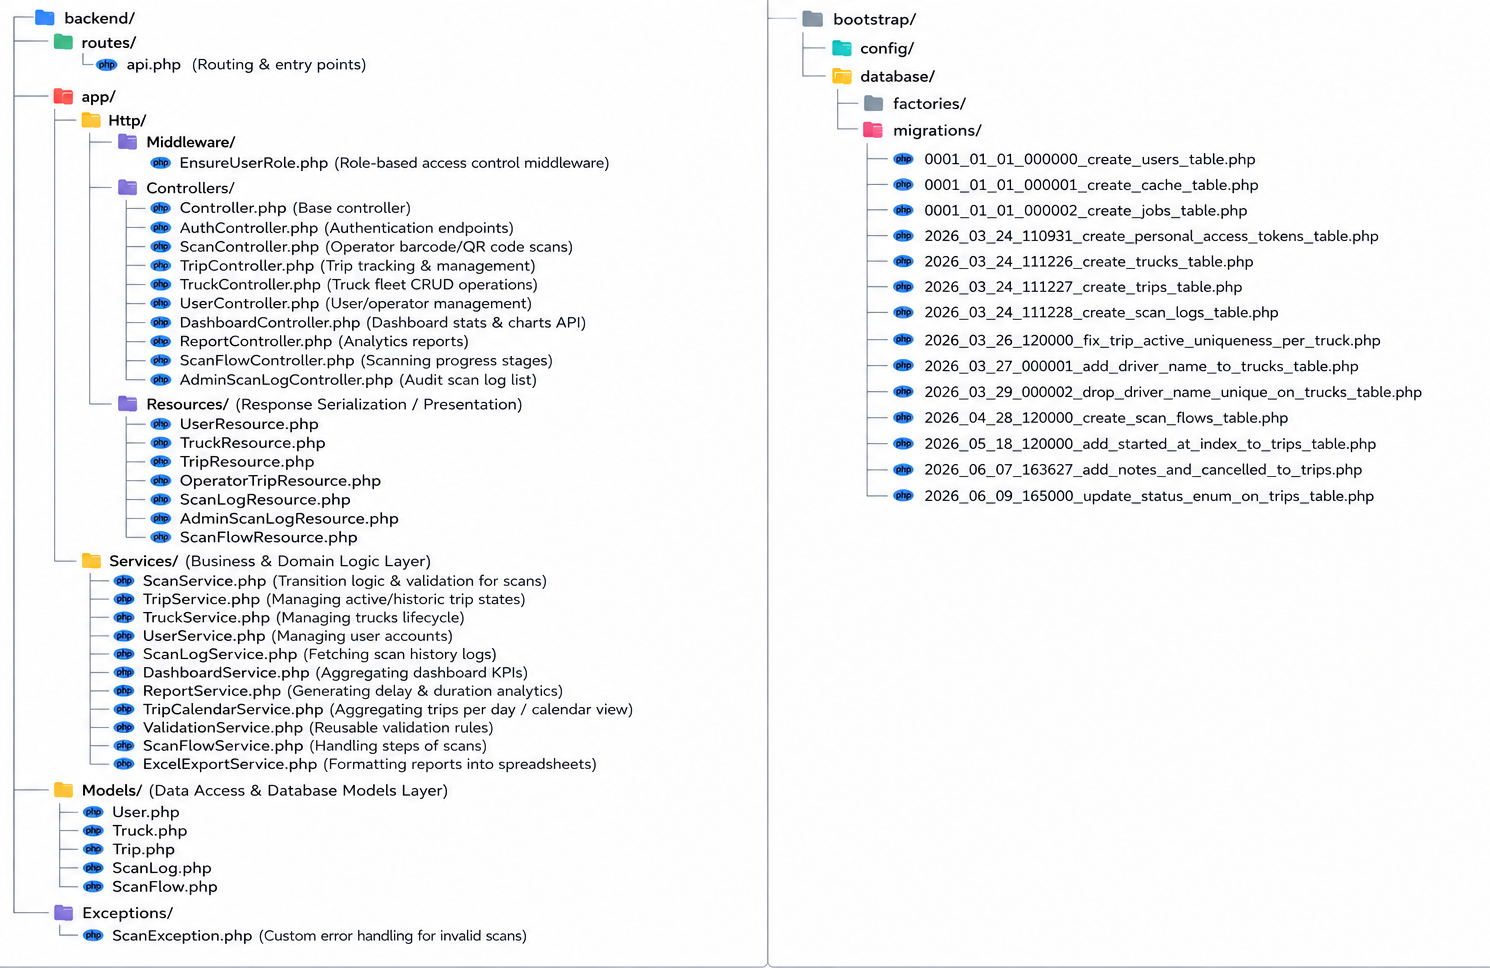
\includegraphics[width=\textwidth,keepaspectratio]
    {figures/screenshots/backend-structure-projet.png}

    \caption{Structure du projet backend Laravel}

    \label{fig:backend-structure-projet}
\end{figure}

Les principaux contrôleurs implémentés sont présentés dans le tableau~\ref{tab:controleurs-backend}.

\begin{table}[H]
\centering
\begin{tabularx}{\textwidth}{|>{\raggedright\arraybackslash}p{4.2cm}|X|}
\hline
\textbf{Contrôleur} & \textbf{Rôle principal} \\
\hline
{\scriptsize\codepath{AuthController.php}} & Gérer la connexion, la récupération du profil courant et la déconnexion. \\
\hline
{\scriptsize\codepath{ScanController.php}} & Recevoir les scans QR envoyés par l'application mobile et déclencher le traitement métier. \\
\hline
{\scriptsize\codepath{TruckController.php}} & Gérer les camions, leur état actif et les informations utilisées pour l'identification QR. \\
\hline
{\scriptsize\codepath{TripController.php}} & Gérer les trajets, leurs statuts, leurs détails, les notes et les annulations. \\
\hline
{\scriptsize\codepath{UserController.php}} & Gérer les utilisateurs et les opérateurs. \\
\hline
{\scriptsize\codepath{AdminScanLogController.php}} & Permettre la consultation des logs de scan depuis l'administration. \\
\hline
{\scriptsize\codepath{DashboardController.php}} & Fournir les indicateurs nécessaires au tableau de bord. \\
\hline
{\scriptsize\codepath{ReportController.php}} & Générer les rapports et déclencher les exports. \\
\hline
{\scriptsize\codepath{ScanFlowController.php}} & Gérer la configuration du flux de scan. \\
\hline
\end{tabularx}
\caption{Contrôleurs principaux du backend}
\label{tab:controleurs-backend}
\end{table}

Les modèles principaux sont \texttt{User}, \texttt{Truck}, \texttt{Trip}, \texttt{ScanLog} et \texttt{ScanFlow}. Ils correspondent aux entités métier décrites dans la conception de la base de données. Les tables principales créées par les migrations sont \path{users}, \path{trucks}, \path{trips}, \path{scan_logs}, \path{scan_flows} et \path{personal_access_tokens}. Des tables techniques comme \path{cache} et \path{jobs} sont également présentes pour le fonctionnement interne de Laravel.

\subsection*{Services métier}

La logique métier n'est pas placée directement dans les contrôleurs. Elle est isolée dans des services afin de rendre le code plus maintenable. Les principaux services implémentés sont notamment \texttt{ScanService}, \texttt{ScanFlowService}, \texttt{ValidationService}, \texttt{TripService}, \texttt{TruckService}, \texttt{UserService}, \texttt{ScanLogService}, \texttt{DashboardService}, \texttt{ReportService}, \texttt{TripCalendarService} et \texttt{ExcelExportService}.

Cette séparation permet à chaque service de traiter une responsabilité précise. Par exemple, \texttt{ScanService} orchestre le traitement d'un scan, \texttt{ScanFlowService} détermine l'étape attendue dans le cycle de scan, \texttt{ValidationService} vérifie les règles métier, tandis que \texttt{ExcelExportService} gère la génération des fichiers d'export.

\subsection*{Gestion des camions et des QR codes}

La gestion des camions permet à l'agent logistique d'enregistrer les véhicules utilisés pour les trajets entre l'usine et le port. Chaque camion possède un numéro d'immatriculation unique et une valeur d'identification utilisée lors du scan.

Il est important de distinguer deux aspects. Le backend conserve les données nécessaires à l'identification du camion et vérifie l'unicité des informations. En revanche, la génération visuelle du QR code imprimable est réalisée côté application web, à l'aide des bibliothèques \texttt{qrcode} et \texttt{jsPDF}. L'agent logistique peut ainsi télécharger un document contenant le QR code pour l'imprimer et l'attacher au camion.

\begin{figure}[H]
    \centering
    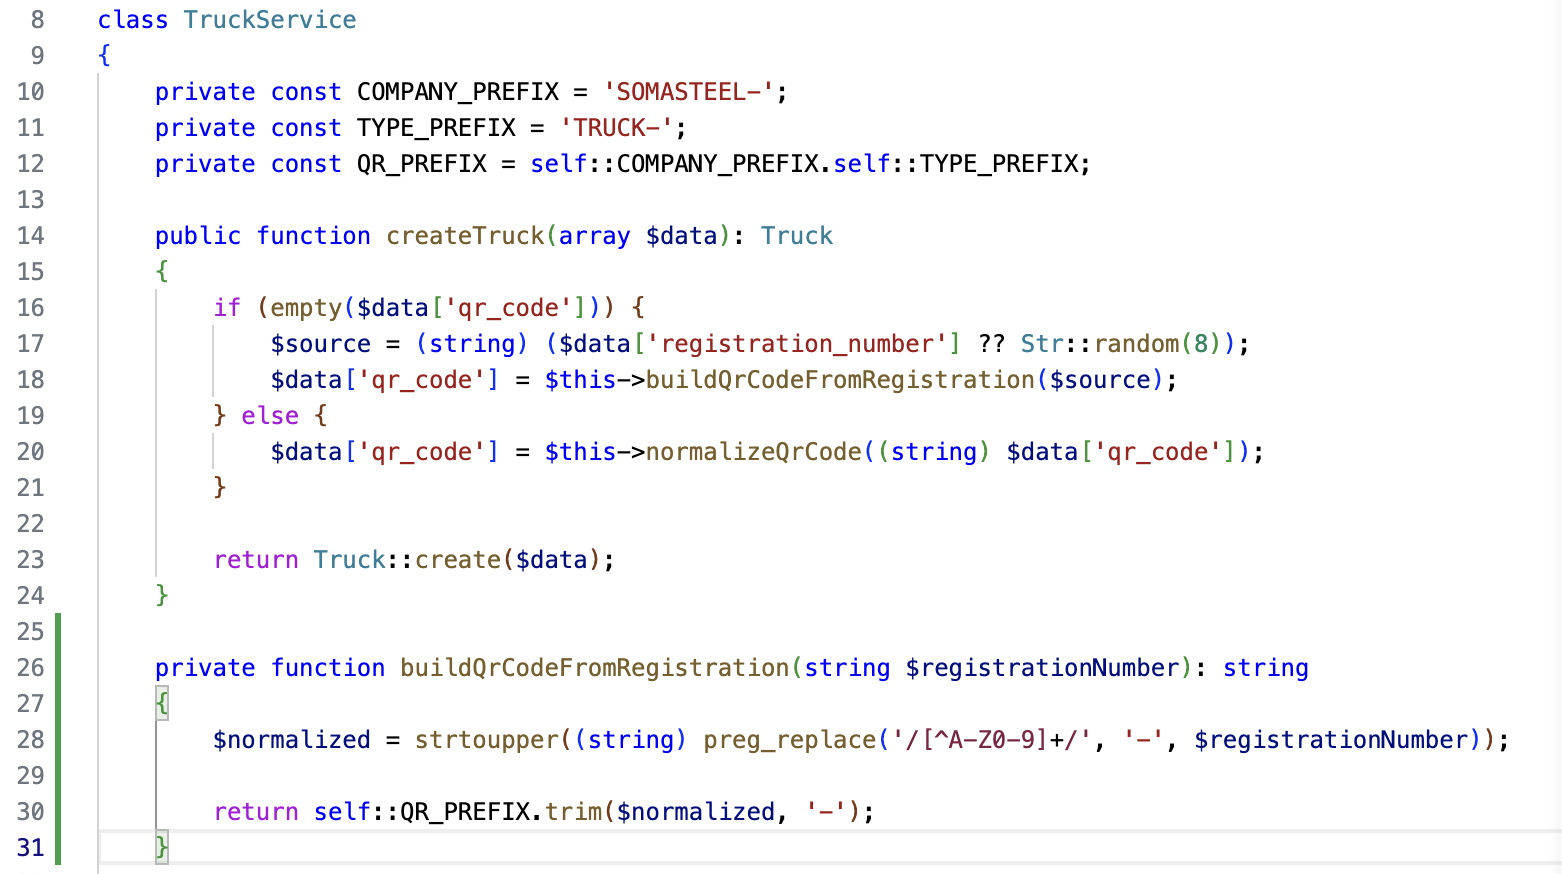
\includegraphics[width=\textwidth,keepaspectratio]
    {figures/screenshots/backend-generation-qr-code.png}

    \caption{Exemple de génération de QR code}

    \label{fig:backend-generation-qr-code}
\end{figure}

\subsection*{Traitement du scan QR}

Le traitement du scan constitue le module métier principal du backend. Lorsqu'un opérateur scanne un camion depuis l'application mobile, le backend reçoit le contenu du QR code ainsi que les informations nécessaires à la validation de la requête.

Le traitement réalisé par \texttt{ScanService} suit les étapes suivantes :

\begin{enumerate}
    \item recevoir la valeur du QR code et l'utilisateur authentifié ;
    \item extraire les candidats possibles à partir du contenu scanné ;
    \item rechercher le camion correspondant dans la base de données ;
    \item vérifier que le camion est actif ;
    \item rechercher le trajet actif associé au camion ;
    \item déterminer la prochaine étape attendue à l'aide de \texttt{ScanFlowService} ;
    \item valider l'action avec \texttt{ValidationService} ;
    \item créer un nouveau trajet ou mettre à jour le trajet existant ;
    \item créer un log de scan ;
    \item déclencher l'événement correspondant au nouveau statut du trajet ;
    \item construire et retourner la réponse API.
\end{enumerate}

En cas de succès, la réponse contient le statut courant, la prochaine étape attendue et un résumé du trajet. En cas d'erreur, par exemple si le camion est introuvable ou si l'action est refusée, le backend retourne un message explicite avec un code HTTP adapté.

\subsection*{Authentification et contrôle des rôles}

L'authentification du backend repose sur Laravel Sanctum. Les routes protégées utilisent le middleware \texttt{auth:sanctum}. Le contrôle d'accès par rôle est assuré par un middleware dédié, \texttt{EnsureUserRole}, qui limite les actions selon le profil connecté.

Cette implémentation permet de séparer l'authentification, qui vérifie l'identité de l'utilisateur, et l'autorisation, qui vérifie si l'utilisateur possède le droit d'exécuter une action. Les validations métier du scan complètent ce contrôle en vérifiant également la localisation et l'étape attendue.

\subsection*{Rapports et exports}

Les fonctionnalités de reporting sont implémentées à travers \texttt{ReportController.php}, \texttt{ReportService.php} et \texttt{ExcelExportService.php}. Elles permettent de produire des synthèses, des rapports par camion, des rapports de durée, des analyses de retard et des exports exploitables par l'agent logistique.

\section{Implémentation frontend}

La partie frontend de SomaScan est composée de deux applications distinctes : une application mobile pour les opérateurs terrain et une application web pour l'agent logistique. Ces deux interfaces consomment les API exposées par le backend, mais elles répondent à des besoins différents.

\subsection{Application mobile avec Flutter}

L'application mobile est destinée aux opérateurs de l'usine et du port. Elle a été conçue pour rester simple et rapide à utiliser, car les opérations de scan se déroulent dans un contexte terrain. Les fonctionnalités principales sont l'authentification, l'affichage de l'état de session, la lecture du QR code, l'envoi du scan au backend et l'affichage du résultat.

L'application utilise Flutter et Dart. Elle est organisée autour de modules fonctionnels, notamment l'authentification, le tableau de bord opérateur et le scan. La gestion d'état repose sur Riverpod, le routage est assuré par GoRouter et les appels HTTP sont réalisés avec Dio.

\begin{figure}[H]
    \centering
    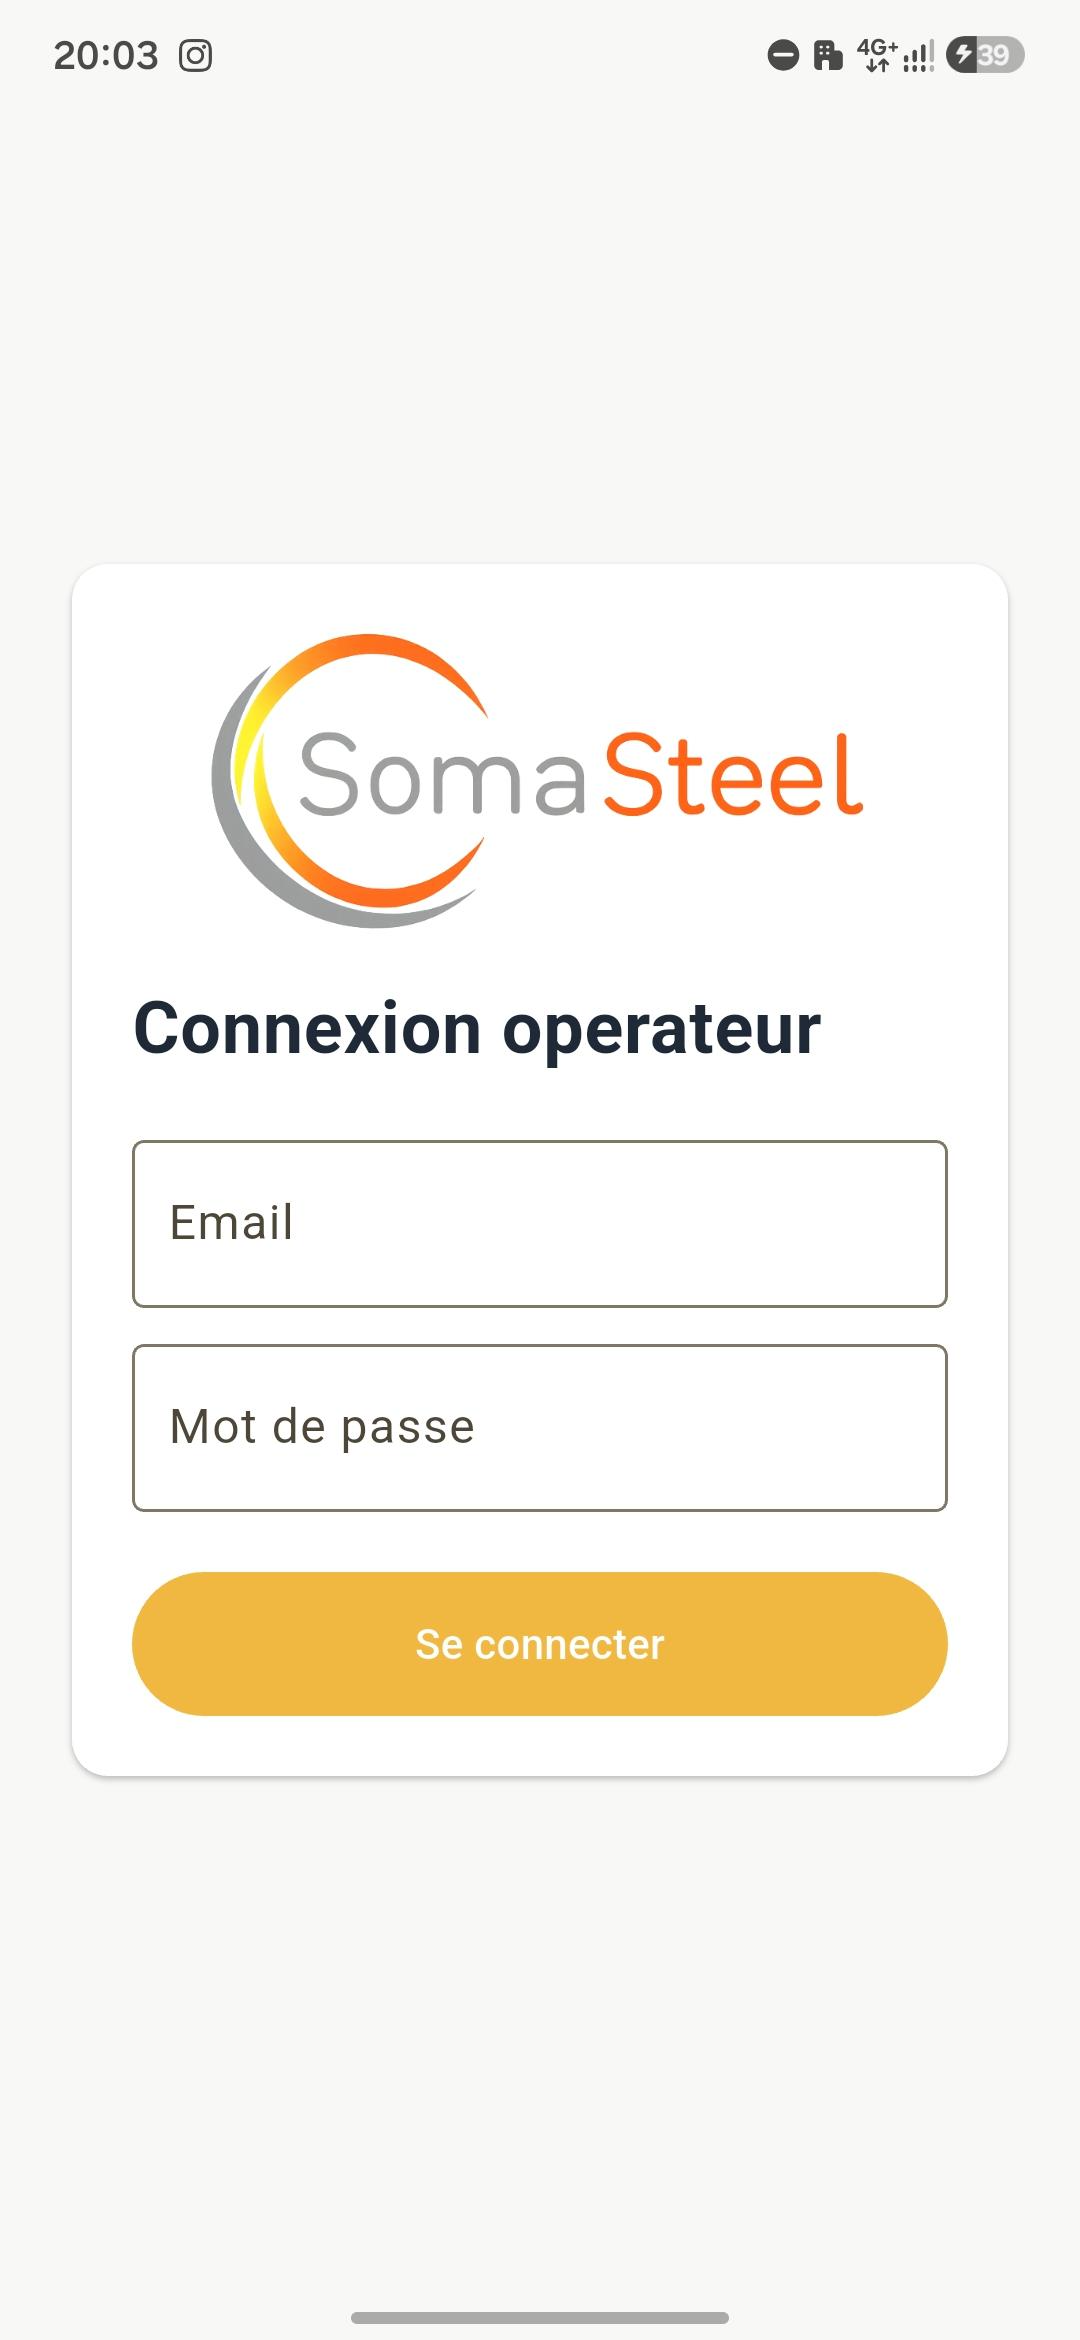
\includegraphics[width=\textwidth,height=0.82\textheight,keepaspectratio]
    {figures/screenshots/mobile-login.png}

    \caption{Écran de connexion mobile}

    \label{fig:mobile-login}
\end{figure}

La configuration de l'URL de l'API est réalisée à l'aide de constantes de compilation Dart. La variable \path{API_BASE_URL} permet de définir l'adresse du backend. Par défaut, l'application peut viser l'API distante, mais il est possible de la lancer vers un backend local avec une option de type \texttt{--dart-define}.

L'application nécessite également les permissions liées à son fonctionnement. L'accès à la caméra est indispensable pour lire les QR codes avec le module de scan, et l'accès Internet est nécessaire pour communiquer avec l'API backend.

Le module de scan utilise la caméra du téléphone pour lire le QR code du camion. Après lecture, l'application envoie la valeur capturée au backend avec les informations nécessaires, comme l'heure du périphérique et l'identifiant de l'appareil lorsque disponible. La réponse du backend indique si le scan est accepté ou refusé.

\begin{figure}[H]
    \centering
    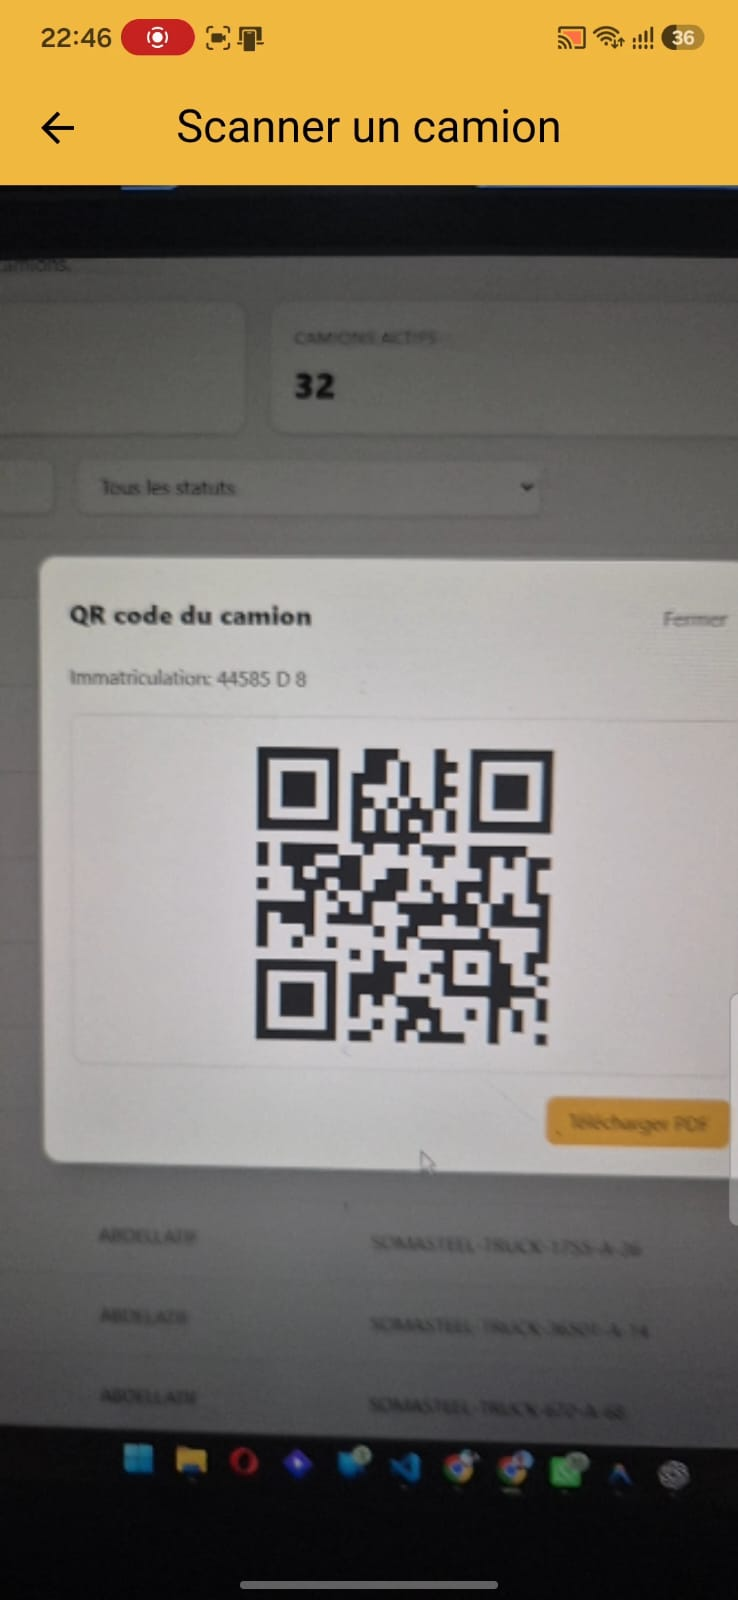
\includegraphics[width=\textwidth,height=0.82\textheight,keepaspectratio]
    {figures/screenshots/mobile-scan-qr.png}

    \caption{Écran de scan QR mobile}

    \label{fig:mobile-scan-qr}
\end{figure}

Après chaque opération, l'application affiche un retour clair à l'opérateur. En cas de succès, elle indique le statut mis à jour ou l'action enregistrée. En cas d'erreur, elle affiche le message retourné par le backend afin de permettre à l'opérateur de comprendre la cause du refus.

\begin{figure}[H]
    \centering
    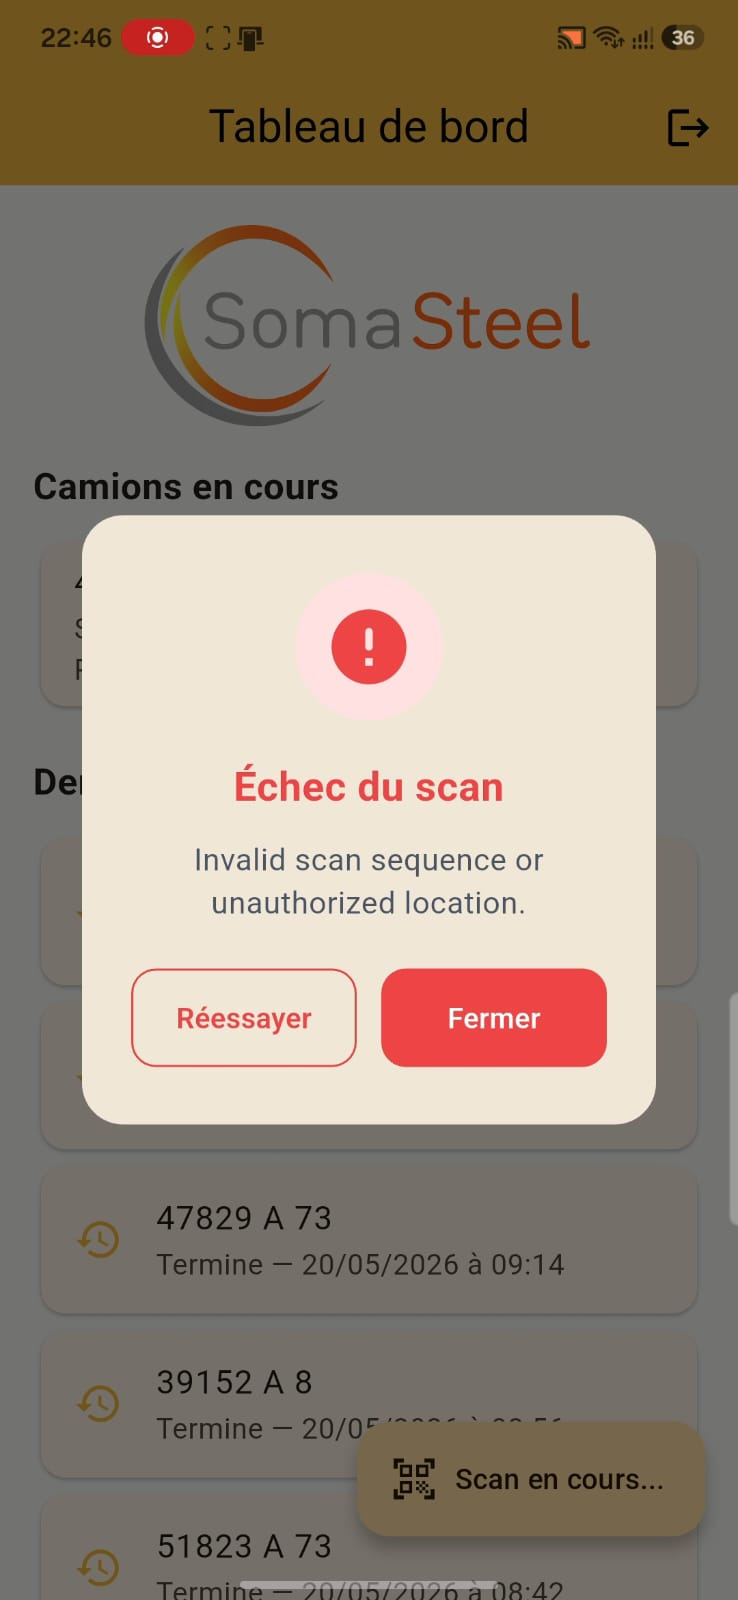
\includegraphics[width=\textwidth,height=0.82\textheight,keepaspectratio]
    {figures/screenshots/mobile-resultat-scan.png}

    \caption{Écran résultat du scan et statut mis à jour}

    \label{fig:mobile-resultat-scan}
\end{figure}

\subsection{Application web avec React}

L'application web est destinée à l'agent logistique. Elle fournit une interface d'administration et de supervision permettant de gérer les données, de suivre les trajets et de consulter l'activité logistique sous forme de tableaux de bord. Elle est développée sous forme d'application monopage avec React, TypeScript et Vite.

Le dossier \codepath{src/} est organisé par responsabilités. Le dossier \codepath{api/} contient les modules de communication avec le backend et l'instance Axios. Le dossier \codepath{components/} regroupe les composants réutilisables. Le dossier \codepath{layouts/} contient la structure générale du back-office. Le dossier \codepath{pages/} contient les écrans principaux. Le dossier \codepath{routes/} contient la configuration du routage et les routes protégées. Le dossier \codepath{store/} contient l'état global, notamment \codepath{authStore.ts}.

Les routes principales implémentées sont la page de connexion, le tableau de bord, la gestion des camions, la gestion des utilisateurs, la liste des trajets, le détail d'un trajet et la vue calendrier des trajets. Des pages d'erreur permettent également de gérer les routes inexistantes ou les accès non autorisés.

Le tableau de bord permet de visualiser les indicateurs principaux liés aux trajets, aux camions et aux scans. Il donne à l'agent logistique une vue synthétique de l'activité et facilite le suivi opérationnel.

\begin{figure}[H]
    \centering
    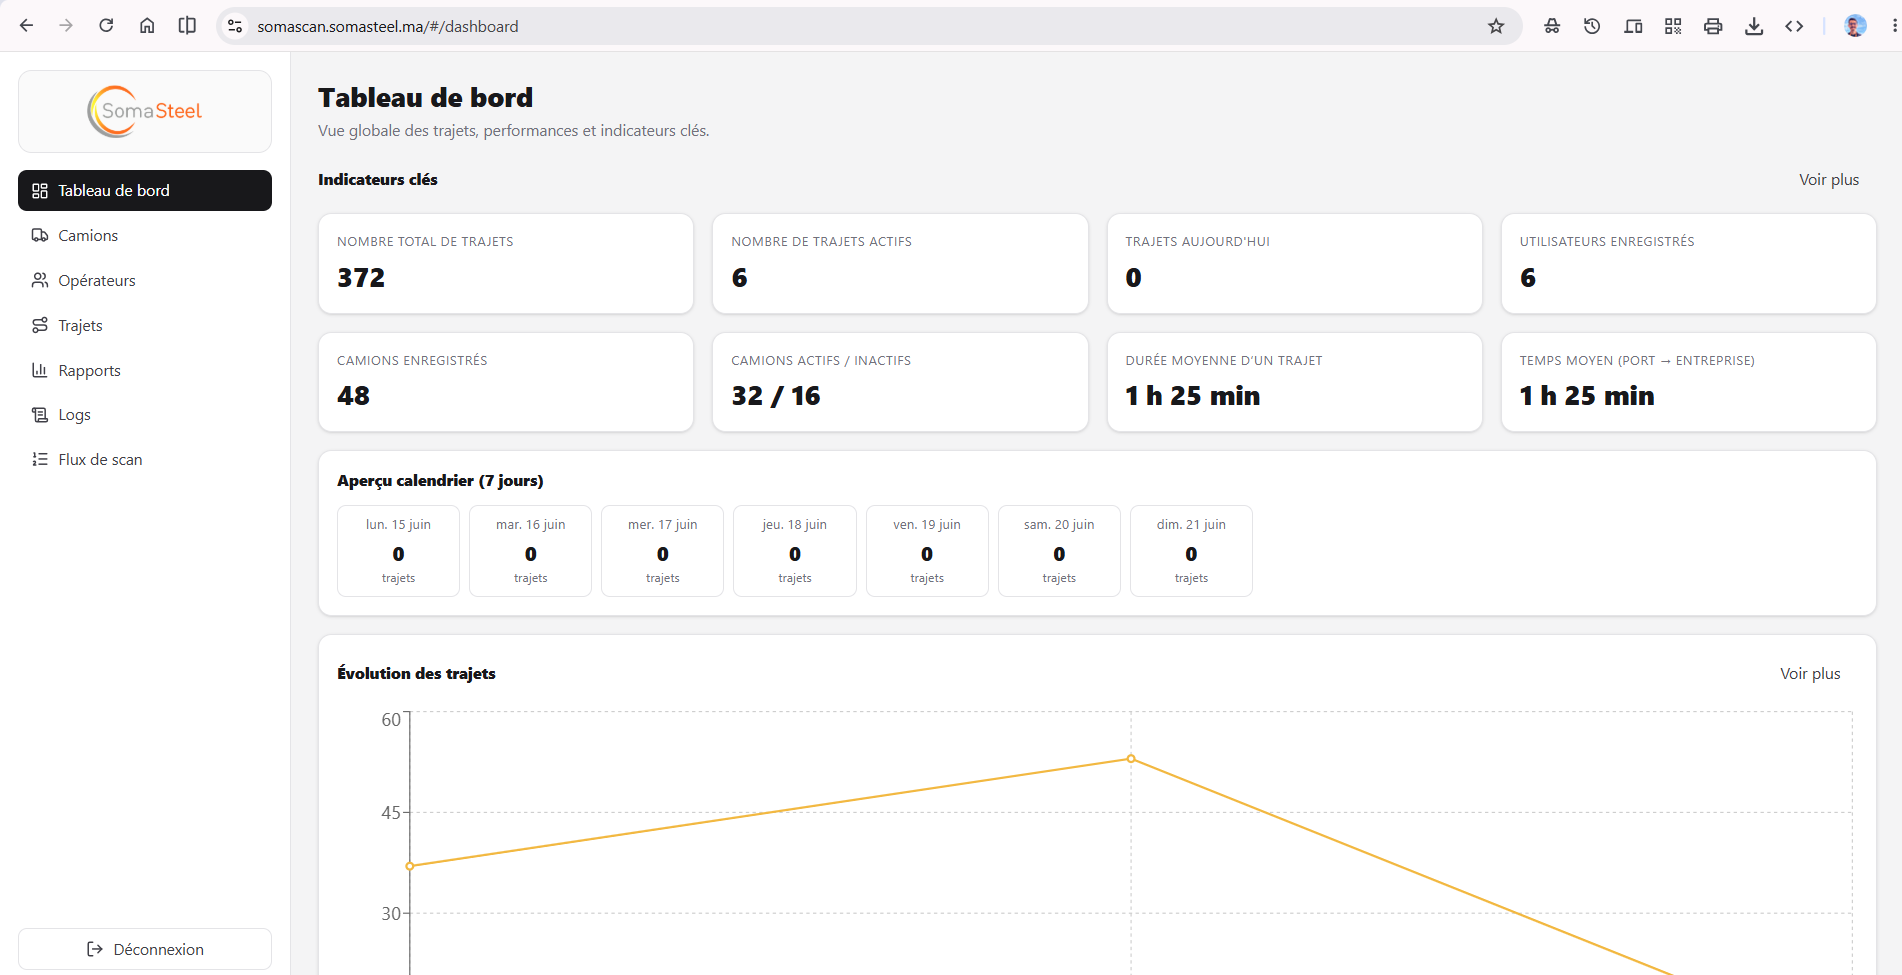
\includegraphics[width=\textwidth,keepaspectratio]
    {figures/screenshots/web-dashboard-expeditions.png}

    \caption{Dashboard web de suivi des expéditions}

    \label{fig:web-dashboard-expeditions}
\end{figure}


La gestion des camions permet d'ajouter, de modifier, d'activer ou de désactiver les véhicules suivis par le système. Elle inclut également la génération et le téléchargement du QR code imprimable depuis l'interface web.

\begin{figure}[H]
    \centering
    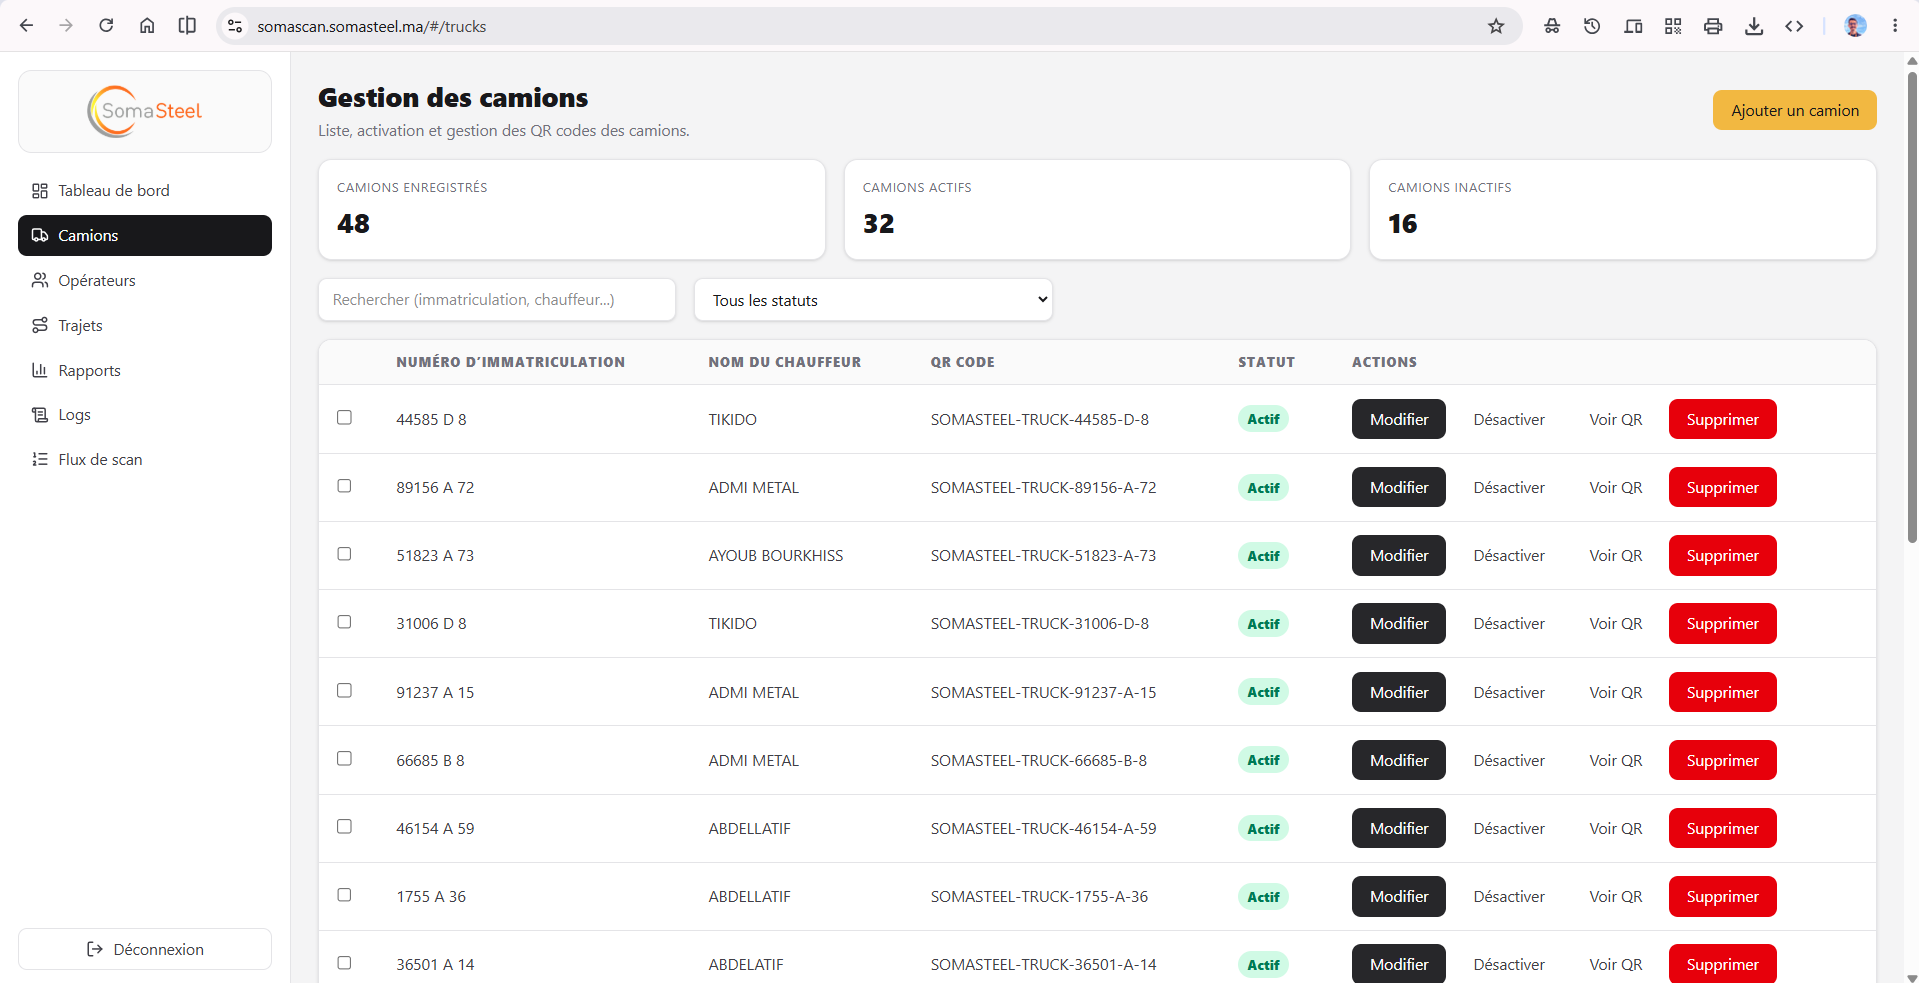
\includegraphics[width=\textwidth,keepaspectratio]
    {figures/screenshots/web-gestion-camions.png}

    \caption{Interface gestion des camions}

    \label{fig:web-gestion-camions}
\end{figure}

Lors de l'ajout d'un camion, l'application web utilise les données du camion pour générer un QR code. Le document peut ensuite être téléchargé au format PDF afin d'être imprimé et utilisé physiquement sur le camion.

\begin{figure}[H]
    \centering
    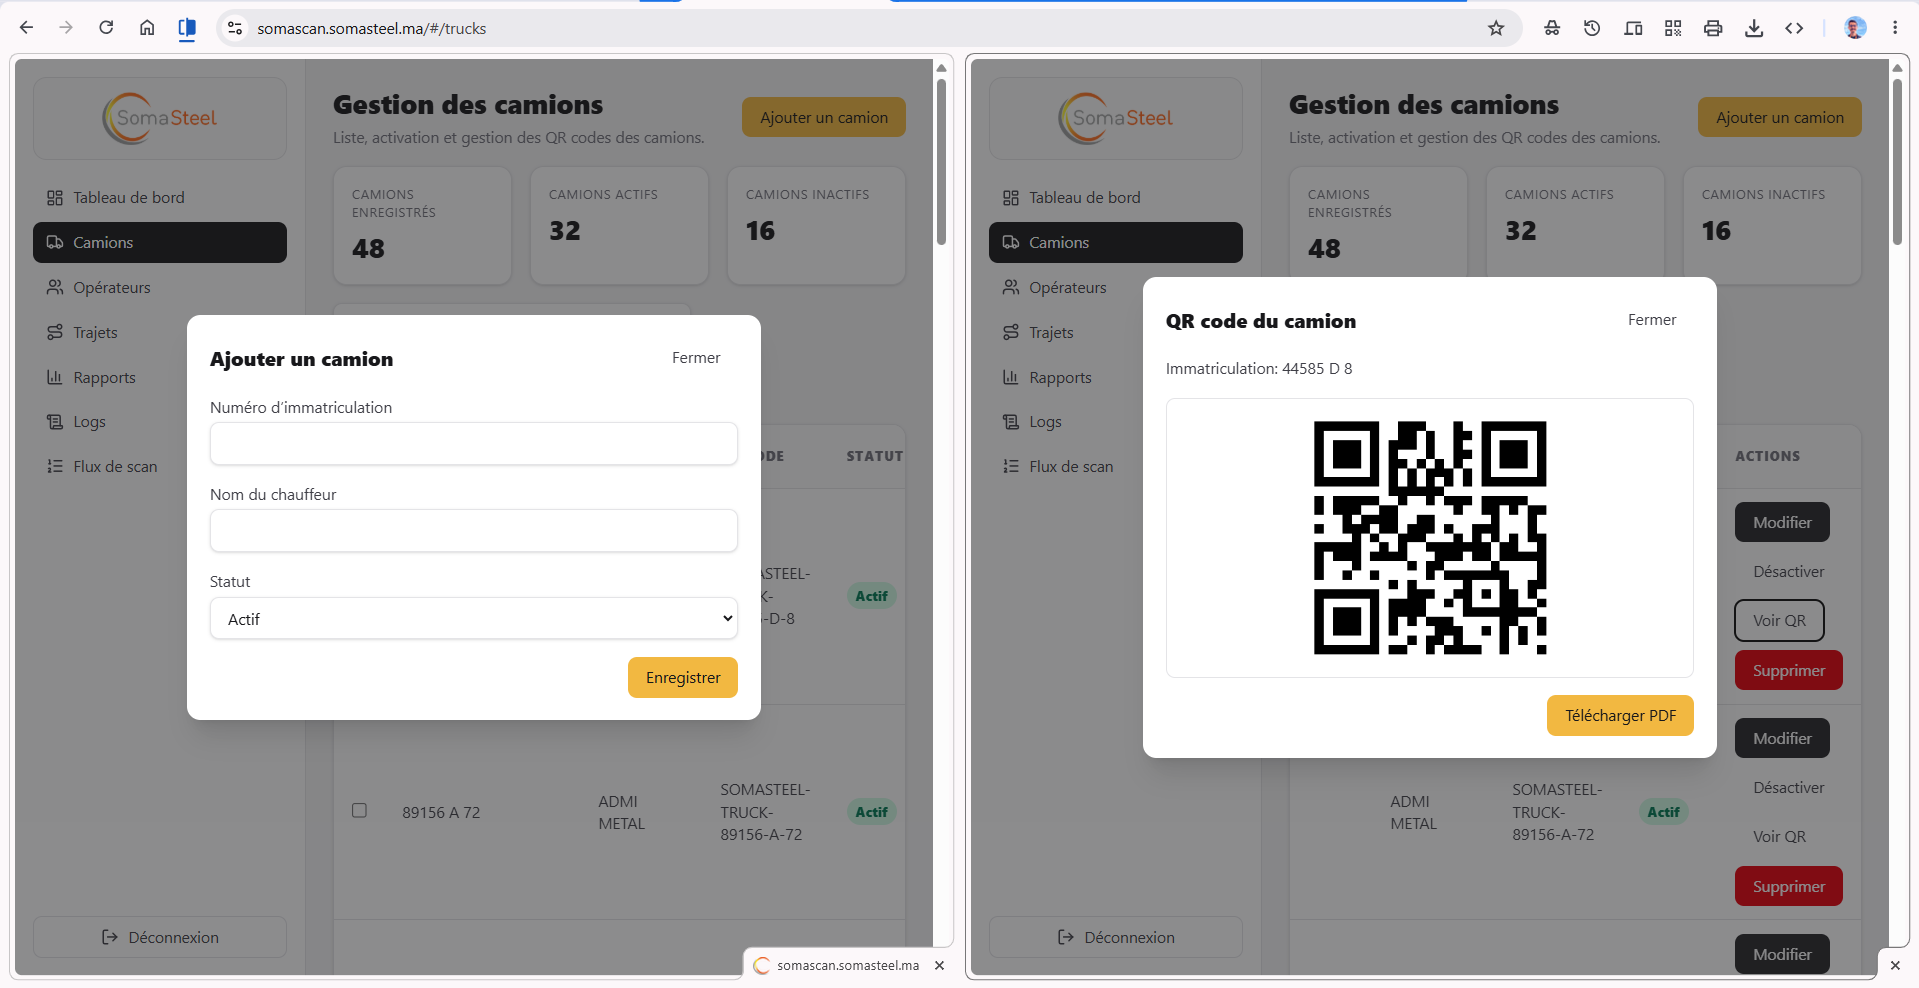
\includegraphics[width=\textwidth,keepaspectratio]
    {figures/screenshots/web-ajout-camion-qr.png}

    \caption{Interface ajout camion et téléchargement QR code}

    \label{fig:web-ajout-camion-qr}
\end{figure}

L'application web contient également une vue calendrier destinée au suivi mensuel des trajets. Cette interface présente les jours du mois sous forme de calendrier et affiche, pour chaque journée, des indicateurs opérationnels tels que le nombre de trajets réalisés, terminés ou encore actifs. Cette vue permet à l'agent logistique d'obtenir une lecture rapide de l'activité sur une période donnée, sans devoir parcourir uniquement une liste tabulaire.

\begin{figure}[H]
    \centering
    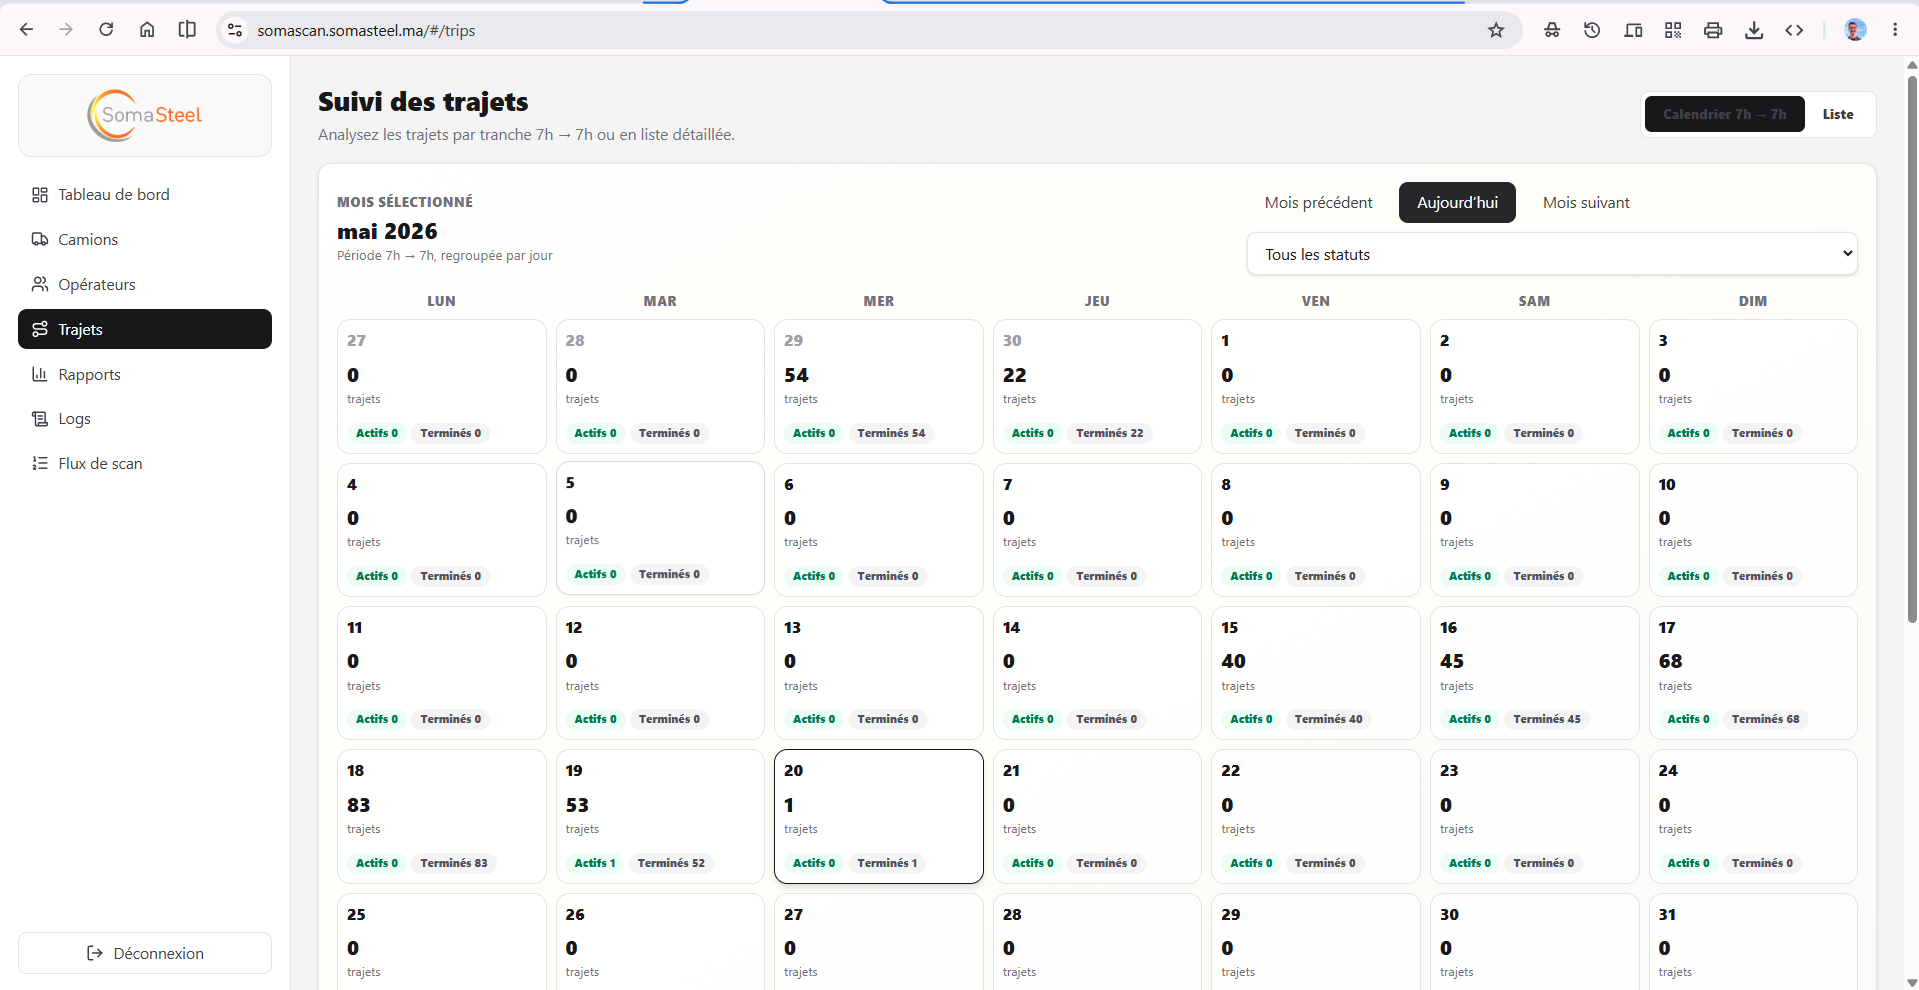
\includegraphics[width=\textwidth,keepaspectratio]
    {figures/screenshots/web-calendrier-trajets.png}

    \caption{Vue calendrier mensuelle des trajets}

    \label{fig:web-calendrier-trajets}
\end{figure}

\section{Intégration API et authentification}

L'intégration entre les trois parties de SomaScan repose sur des API REST exposées par le backend. Les applications mobile et web envoient des requêtes HTTP au format JSON et reçoivent des réponses normalisées contenant les données, un message de résultat et, le cas échéant, des erreurs de validation.

Du côté web, l'instance Axios ajoute automatiquement le jeton d'authentification dans l'en-tête \texttt{Authorization}. Un intercepteur de réponse permet de détecter les erreurs \texttt{401 Unauthorized}. Dans ce cas, la session locale est supprimée et l'utilisateur est redirigé vers la page de connexion.

Du côté mobile, Dio est utilisé pour envoyer les requêtes au backend. Le jeton est conservé dans un stockage sécurisé afin de protéger la session de l'utilisateur. Lorsqu'un opérateur effectue une action protégée, le jeton est joint à la requête afin que le backend puisse identifier l'utilisateur.

Le backend vérifie chaque requête protégée à l'aide de Laravel Sanctum. Les middlewares contrôlent ensuite le rôle de l'utilisateur afin de déterminer s'il peut accéder à la ressource demandée. Ce contrôle est complété par des validations métier, notamment lors des scans, afin de vérifier que l'utilisateur dispose du rôle et de la localisation compatibles avec l'action demandée.

\section{Tests et interfaces principales}

Les tests réalisés visent à vérifier le bon fonctionnement des fonctionnalités principales. Ils concernent notamment l'authentification, la gestion des camions, la génération des QR codes, l'exécution du cycle de scan, le rejet des actions invalides, la consultation des trajets et la génération des rapports.

Les endpoints API peuvent être testés avec un outil de requêtes HTTP afin de vérifier les réponses du backend, les statuts retournés et les messages d'erreur. Ces tests permettent de valider séparément la logique backend avant de vérifier son intégration complète avec les interfaces mobile et web.

\artifactplaceholder
{Test API avec Postman ou outil équivalent}
{fig:test-api-postman}
{figures/screenshots/test-api-postman.png}

Un scénario fonctionnel complet consiste à enregistrer un camion, générer son QR code depuis l'application web, démarrer un trajet depuis l'usine, enregistrer son arrivée au port, enregistrer son départ du port puis clôturer le trajet lors du retour à l'usine. Ce scénario permet de vérifier la cohérence du cycle de vie d'une expédition et la création des logs associés.

\begin{figure}[H]
    \centering
    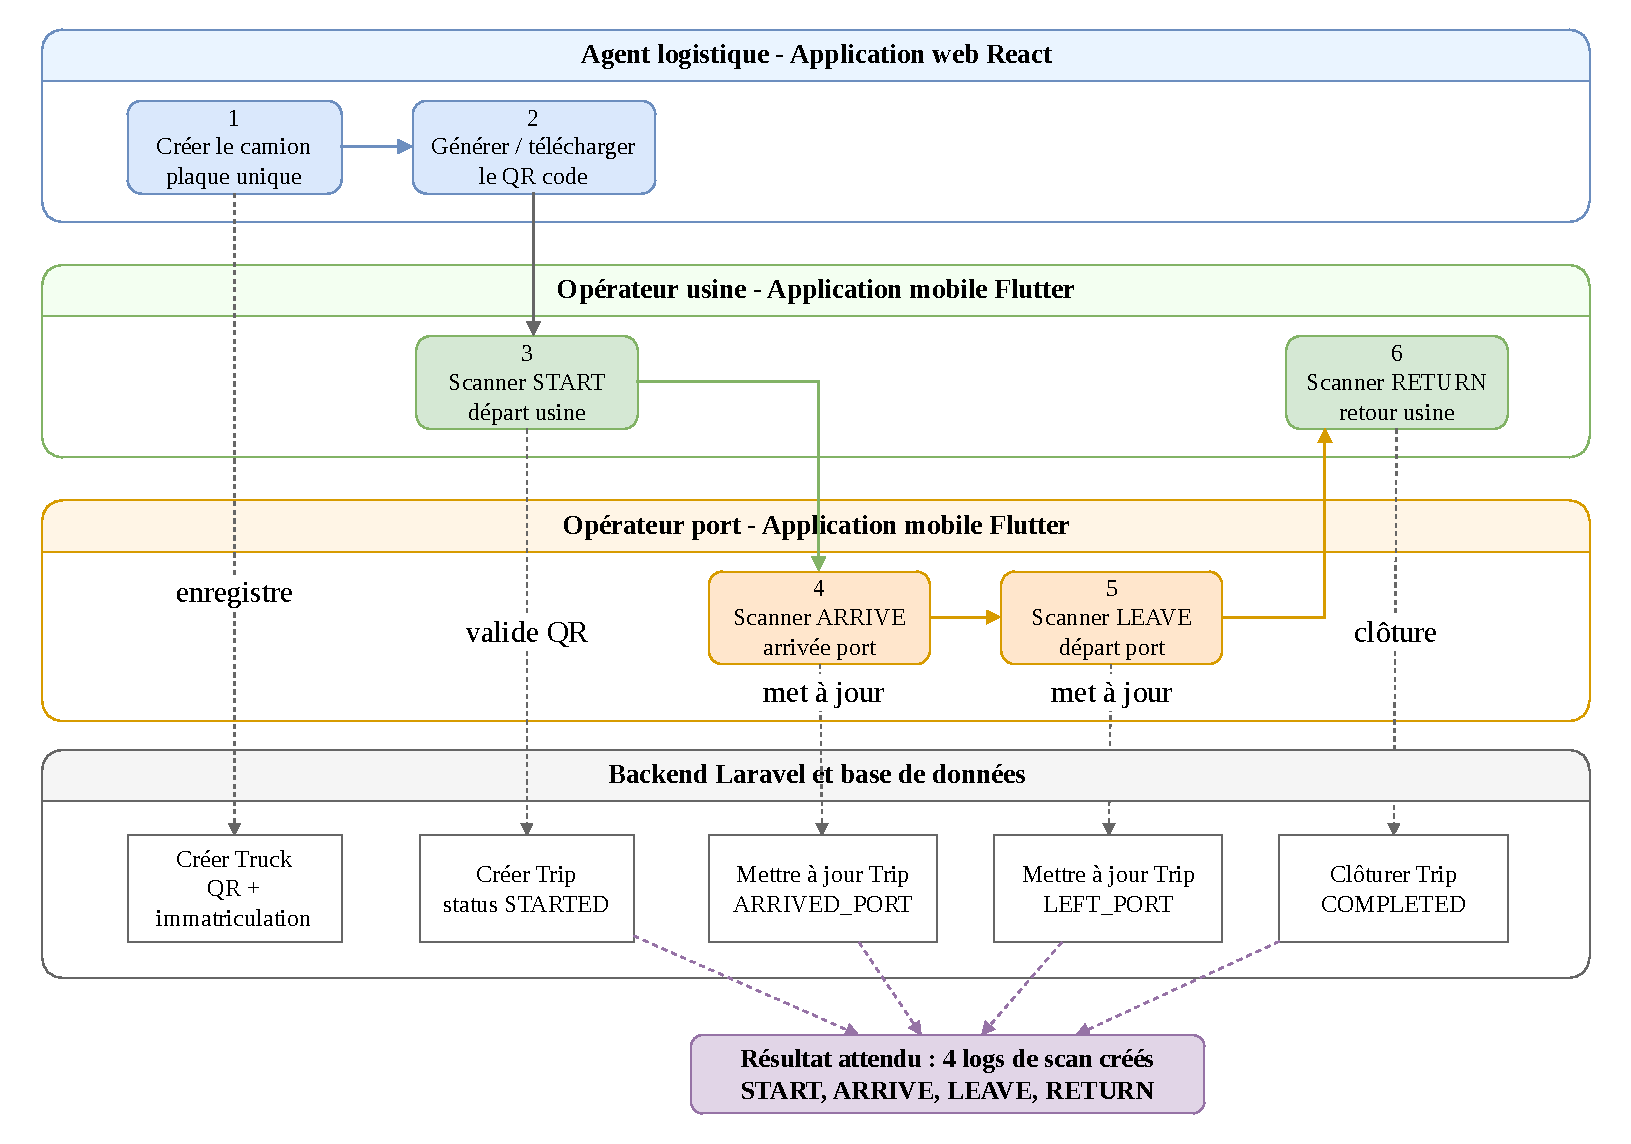
\includegraphics[width=\textwidth,keepaspectratio]
    {figures/diagrams/scenario-test-scan.pdf}

    \caption{Exemple de test fonctionnel scan port vers usine}

    \label{fig:scenario-test-scan}
\end{figure}

\section{Conclusion}

Ce chapitre a présenté la mise en œuvre technique de SomaScan. Le backend Laravel assure la logique métier, l'exposition des API, l'authentification, la gestion des rôles et la persistance des données. L'application mobile Flutter permet aux opérateurs terrain d'effectuer les scans QR et de recevoir un retour immédiat. L'application web React fournit à l'agent logistique les interfaces nécessaires à l'administration, au suivi, à la génération des QR codes et au reporting.

L'implémentation réalisée permet de répondre aux besoins définis dans les chapitres précédents. Elle assure l'identification des camions, le suivi des expéditions par scans successifs, la traçabilité des opérations et la supervision des activités logistiques. Le chapitre suivant sera consacré au déploiement de la solution et à l'organisation DevOps proposée.
